\documentclass[aspectratio=43]{beamer}
\usepackage{luatexja-fontspec}
\usepackage{graphicx,color,multicol,verbatim,listingsutf8}
\usepackage{xcolor}
\usepackage{url}
\usepackage[symbol]{footmisc}
\usetheme{Boadilla}
\usecolortheme[RGB={140,0,0}]{structure}
\setbeamertemplate{navigation symbols}{}
\setbeamercovered{transparent}
\usefonttheme{professionalfonts}
\renewcommand\familydefault{\rmdefault}
\renewcommand{\figurename}{図\thefigure}
\renewcommand{\thefootnote}{\fnsymbol{footnote}}
\setbeamertemplate{sections/subsections in toc}[sections numbered]
\setbeamertemplate{enumerate item}[default]
\setbeamertemplate{itemize item}[triangle]
\lstset{
        %枠外に行った時の自動改行
    breaklines = true,
        %自動改行後のインデント量(デフォルトでは20[pt])
    breakindent = 10pt,
        %標準の書体
    basicstyle = \ttfamily\small,
        %コメントの書体
    commentstyle = {\ttfamily \color[cmyk]{1,0.4,1,0}},
        %関数名等の色の設定
    classoffset = 0,
        %キーワード(int, ifなど)の書体
    keywordstyle = {\bfseries\ttfamily \color[cmyk]{0,1,0,0}},
        %表示する文字の書体
    stringstyle = {\ttfamily \color[rgb]{0,0,1}},
        %枠 tは上に線を記載, Tは上に二重線を記載
        %他オプション:leftline,topline,bottomline,lines,single,shadowbox
    frame = single,
        %frameまでの間隔(行番号とプログラムの間)
    framesep = 5pt,
        %行番号の位置
    numbers = left,
        %行番号の間隔
    stepnumber = 1,
        %行番号の書体
    numberstyle = \scriptsize,
        %タブの大きさ
    tabsize = 4,
        %キャプションの場所(tbならば上下両方に記載)
    captionpos = t,
    xleftmargin=1.5em
}
\makeatletter
\title{3. 音声合成}
\subtitle{情報学群実験第3c 3i}
\author{Group 10\thanks{門屋 陽丈\and 谷保 愛華\and 内藤 熙人\and 成岡 小雪\and 平林 里菜\and 三上 柊\and 溝口 洸熙}}
\date{2023.04.20}
\newcommand{\showsec}{\thesection .}
\setbeamercolor{block title}{bg=black,fg=white}
\setbeamercolor{block body}{bg=gray!10,fg=black}
\begin{document}
\begin{frame}
    \titlepage
\end{frame}
\begin{frame}
    \begin{multicols}{2}
        \tableofcontents
    \end{multicols}
\end{frame}
\section{初期位相・矩形波}
\begin{frame}[t]{\showsec 初期位相・矩形波}
    周波数\(f\),時刻を\(t\)に設定する.
    \begin{block}{初期位相}
        初期位相を\(\phi\)に設定する.
        \begin{align}
            y(t) & = \sin(2\pi ft+\phi)
        \end{align}
    \end{block}
    \begin{block}{短形波のフーリエ級数展開}
        \begin{align}
            y(t) & = \sum_{k=1}^{\infty}\dfrac{1}{2k-1}\sin\big(2\pi(2k-1)ft\big)
        \end{align}
    \end{block}
\end{frame}
\section{ノコギリ波}
\begin{frame}[t]{\showsec ノコギリ波}
    \begin{figure}
        \centering
        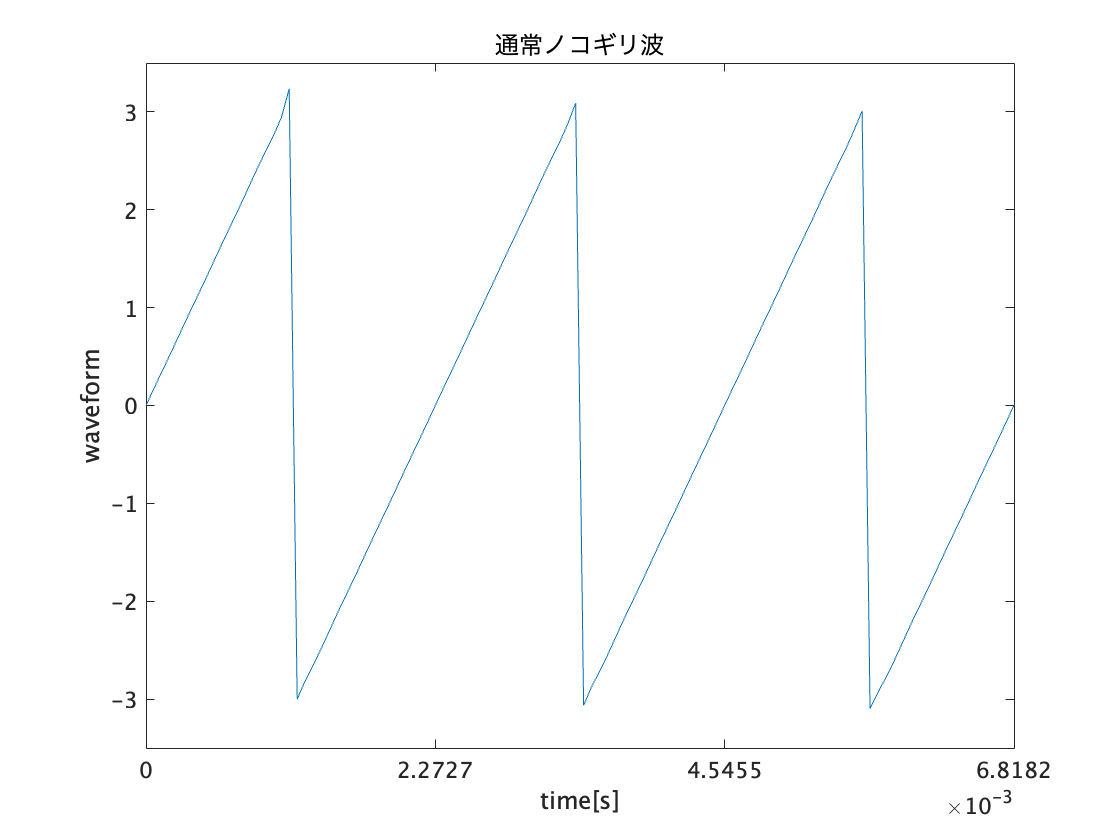
\includegraphics[keepaspectratio,width=0.85\textwidth]{nokogiri.png}
    \end{figure}
\end{frame}
\begin{frame}[t]{\showsec ノコギリ波}
    \begin{align}
        y(t) & =t             & (-\pi<t<\pi)     \\
        \intertext{を周期\(2\pi\)の関数として周期的に拡張したもの.}
        y(t) & = y(t + 2k\pi) & (k\in\mathbb{Z})
    \end{align}
    \begin{block}{ノコギリ波のフーリエ級数展開}
        \begin{align}
            y(t) & =\sum_{k=1}^{\infty}(-1)^{k-1}\dfrac{2}{k}\sin kt
        \end{align}
    \end{block}
    \(\displaystyle\sum_{k=1}^{\infty}\)の\(\infty\)は今回,\texttt{50}としてプログラミングしている.
\end{frame}
\section{課題1}
\subsection{問題}
\begin{frame}[t,containsverbatim]{\showsec 課題1}
    \begin{exampleblock}{}
        矩形波,ノコギリ波を基本周波数 440Hz 等の可聴域の範囲で作成し,さらに各周波数成分も位相を適当な値に変化させよう.\\
        (サンプリング周波数\verb|Fs = 16kHz|,長さ\verb|2s|.)
        \begin{itemize}
            \item 位相の操作
                  \begin{itemize}
                      \item 固定値 \(\pi/4\)
                      \item 固定値 \(\pi/2\)
                      \item ランダム値\footnote{ランダム値は \texttt{variable = rand} で格納できる.}
                  \end{itemize}
        \end{itemize}
    \end{exampleblock}
    \begin{block}{Tips}
        \begin{lstlisting}[language={Matlab},numbers={none},frame={none},xleftmargin=0em]
axis([xmin xmax ymin ymax]);
        \end{lstlisting}
        グラフをプロットするときの範囲を指定できる.周波数\(f\)の周期関数を\texttt{n}周期分プロットしたい場合は\texttt{xmin}を\texttt{0},\texttt{xmax}を\texttt{n/f}に設定する.
    \end{block}
\end{frame}
\subsection{サンプルコード}
\begin{frame}[t,containsverbatim]{\showsec 課題1(サンプルコード)}
    \begin{lstlisting}[language={Matlab}]
clear all;
Fs = 16000; % サンプリング周波数
f = 400;    % 基本周波数
t = [0 : ??] /Fs % 時間軸テーブル
phi1 = pi / 4;   % 初期位相 pi/2
phi2 = pi / 2;   % 初期位相 pi/4
phi3 = rand;     % 初期位相 ランダム
% --- ノコギリ波生成 ---
for k=1:50 % とりあえず50にでも設定しておく
 y1 = ?? + (-1)^(k-1) * 1/3 * 2/k * sin(???);
 y2 = ...;
 y3 = ...;
end
figure;
subplot(?,?,?);
plot(?,?);
...
\end{lstlisting}
\end{frame}
\subsection{結果:ノコギリ波}
\begin{frame}{\showsec 課題1(結果:ノコギリ波)}
    \begin{figure}
        \centering
        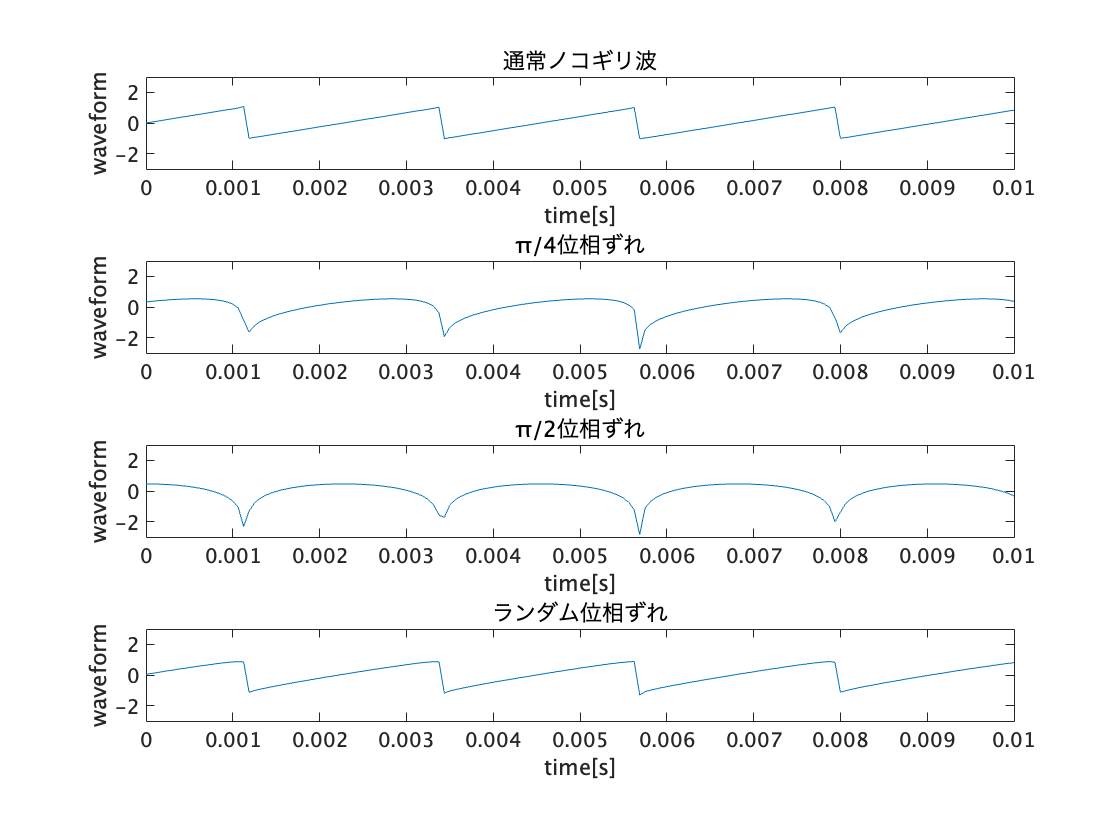
\includegraphics[keepaspectratio,width=0.89\textwidth]{no1_1_ans.png}
    \end{figure}
\end{frame}
\subsection{結果:矩形波}
\begin{frame}{\showsec 課題1(結果:矩形波)}
    \begin{figure}
        \centering
        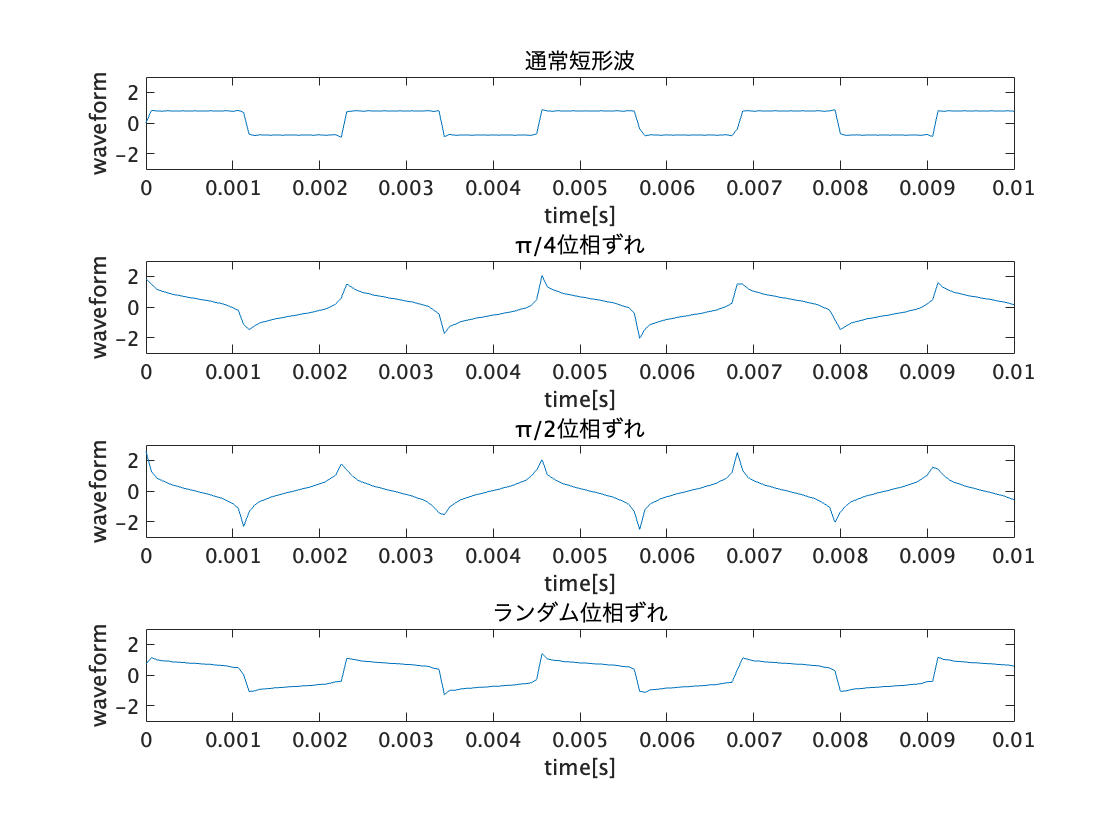
\includegraphics[keepaspectratio,width=0.89\textwidth]{no1_2_ans.png}
    \end{figure}
\end{frame}
\section{課題2}
\subsection{結果}
\begin{frame}[t]{\showsec 課題2}
    \begin{exampleblock}{}
        自分の母音の音声を4s程度ずつ録音し,その音声データの波形の上下を反転さよう.
        元データと反転後のデータを聴き比べよう.
    \end{exampleblock}
    \begin{figure}
        \centering
        \begin{minipage}[t]{0.49\textwidth}
            \centering
            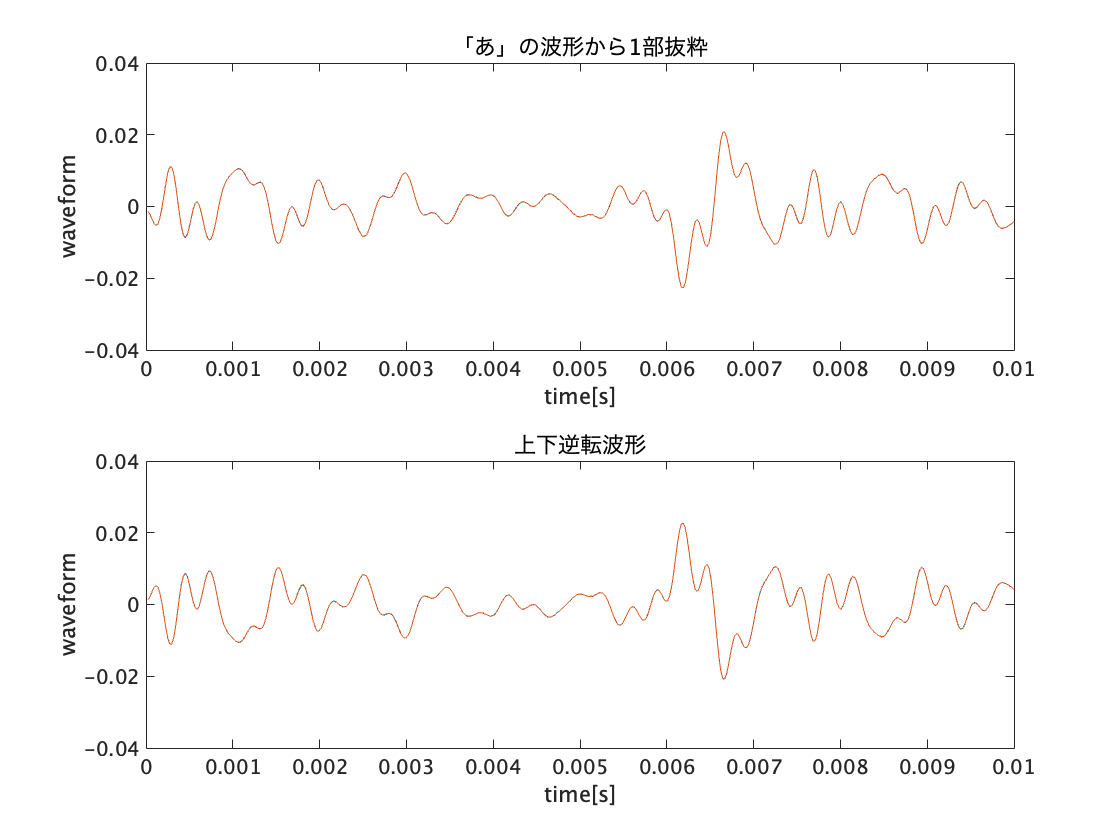
\includegraphics[keepaspectratio,width=\textwidth]{no2_ans.png}
            \caption{それぞれのグラフ}
        \end{minipage}
        \begin{minipage}[t]{0.49\textwidth}
            \centering
            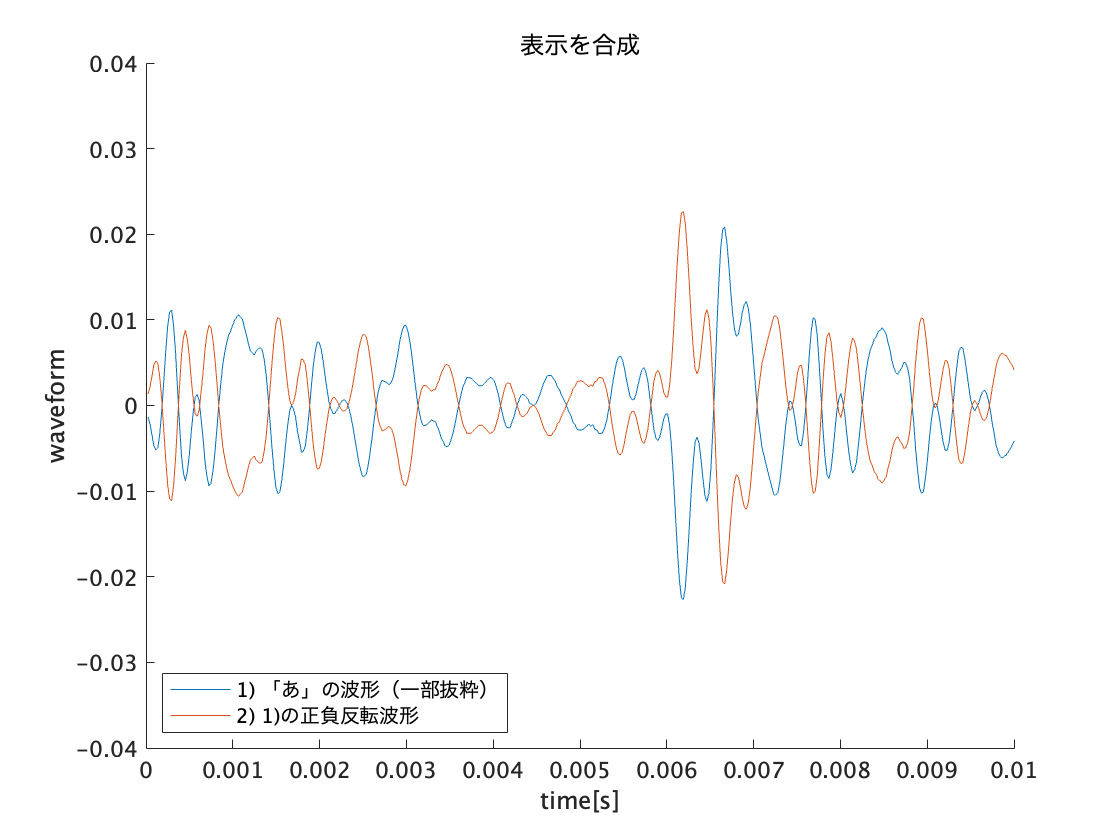
\includegraphics[keepaspectratio,width=\textwidth]{no2_ans_2.png}
            \caption{グラフを重ね合わせてみる}
        \end{minipage}
    \end{figure}
\end{frame}
\subsection{サンプルコード}
\begin{frame}[t,containsverbatim]{\showsec 課題2(サンプルコード)}
    \begin{lstlisting}[language={Matlab}]
clear all;
[y, Fs] = audioread('filename'); %Fs はサンプルレート
N = yの長さ;
t = [1:?]/??; % 音声の流れる時間
for k=1:N
    % 全ての要素数を正ならば負,負ならば正にする.
    z(k) = ??;
end

soundsc(??);

figure;
subplot...
    \end{lstlisting}
\end{frame}
\addtocontents{toc}{\newpage}
\section{周波数解析}
\begin{frame}{\showsec 周波数解析}

\end{frame}
\section{課題3}
\begin{frame}[t]{\showsec 課題3}
    \begin{exampleblock}{}
        \begin{enumerate}
            \item 課題2で録音した各音声を周波数解析し,スペクトル上でピークのある周波数およびその周波数のY軸の値を抽出しよう.
            \item 抽出した周波数,Y軸の値の順音を合成し,音の違いを聴き比べる.
        \end{enumerate}
    \end{exampleblock}
    \dotfill
    \begin{itemize}
        \item 0Hz - 10,000Hz 程度までの範囲で,ピークとなる周波数,及びそのピーク値を高い順から10個程度以上抽出する.\\
              (母音の識別に利用される主な周波数成分は4kHz以下)
        \item 周波数およびピーク値(Y軸の値)は厳密でなくて良い.
        \item \texttt{a},\texttt{i}の合成音の聞こえ方の違い,及び元の音声との違いについて考察する.
    \end{itemize}
\end{frame}
\subsection{サンプルコード}
\begin{frame}[t,containsverbatim]{\showsec 課題3(サンプルコード)}
    \begin{lstlisting}[language=Matlab]
clear all;

\end{lstlisting}
\end{frame}
\end{document}